\documentclass{beamer}
\renewcommand{\baselinestretch}{1.1}
\usepackage{graphicx}
\usepackage{natbib}
\usepackage{amsmath}
\usepackage{hyperref}
\usepackage{listings} 

\def\labelitemi{--}
\parindent=0pt

\usepackage{xcolor}

\colorlet{codecolor}{black!30}
\newcommand{\codebox}[1]{%
  \colorbox{codecolor}{\ttfamily \detokenize{#1}}%
}

\begin{document}
\bibliographystyle{/Users/Lizzie/Documents/EndnoteRelated/Bibtex/styles/besjournals}
\renewcommand{\refname}{\CHead{}}

{\usebackgroundtemplate{%
  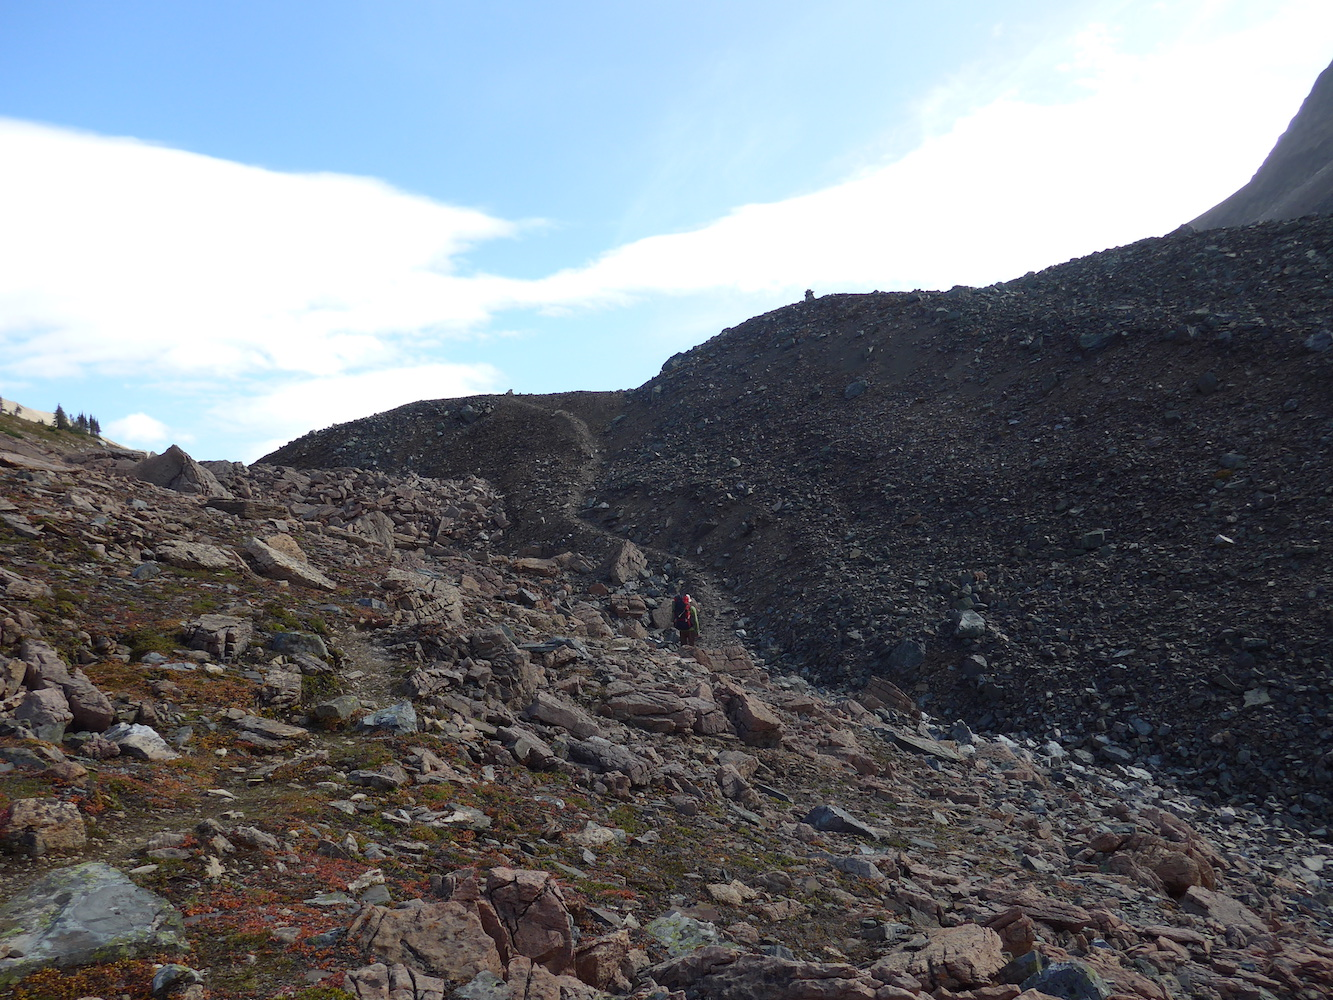
\includegraphics[width=\paperwidth,height=\paperheight]{photo2.jpg}} 
\begin{frame}
\begin{center}
\vspace{35ex}
{\color{white} {\huge Phylogeny model updates}}
\\
\vspace{2ex}
{\color{white} {\Large 7 October 2020}}

\end{center}
\end{frame}
}
	
	\frame{
		\frametitle{What I will cover...}
		\framesubtitle{}
		\begin{itemize}
			\item Review: The way phylogeny is generally handled in ecological statistical models
		\begin{itemize}
                  \item PGLS
                    \item PMM
		\end{itemize}
			\item Review: The way I want to handle it for OSPREE (but I could be wrong)
			\item Review: My progress on that goal (when last we met in June)
                        \item New! My progress on that goal since last met
                          \item New! How you can help!
		\end{itemize}
	}

	\frame{
		\frametitle{A couple quick notes ... }
		\framesubtitle{}
		\begin{itemize}
			\item I am skipping over why we care about phylogeny, check out phylogenyfoundering.pdf for some of that.
                         \item Reminder: Phylogenetic structure in a value (say, a `trait') is measured based on a value called $\lambda$. When $\lambda=1$ the trait is perfectly predicted by the phylogeny; when it's 0, the phylogeny does not matter. 
		\end{itemize}
	}


	\frame{
		\frametitle{Common modeling approaches}
		\framesubtitle{Part 1: PGLS (adapted from second edition of \emph{Statistical Rethinking})}
Consider...
\begin{align}
y & \sim MVN(\mu, S)\\
\mu_i & = \alpha +  \beta*x_i
\end{align}
$\mu$ is a usual linear model. $y$ is a vector of phenological dates (one per species), and $S$ is a covariance matrix with as many rows and columns as species. In ordinary regression this takes the form:
\begin{align}
S = \sigma^2I
\end{align}
where I is just an identity matrix (all 1s) so we can ignore it. 
In PGLS we replace $S$ with the phylogenetic covariance matrix ($\Sigma$). 
	}


	\frame{
		\frametitle{Common modeling approaches}
		\framesubtitle{Part 1: PGLS}
{\bf You have to make sure of a few things}: 
\begin{itemize}
\item Phylogeny must go in as correlation matrix (this makes the diagonals 1s and the off-diagonals the correlation across species due to evolutionary history) and make sure the rows and columns are in the same order as the species will be ordered numerically.
\item This model forces the correlation structure you give it---it does not adjust the correlation structure at all. 
\end{itemize}
If you don't want to assume $\lambda=1$, then you need to estimate a value to multiply the matix by such that:
\begin{align}
S = \sigma^2(\Sigma*\lambda)
\end{align}
	}

	\frame{
		\frametitle{Common modeling approaches}
		\framesubtitle{Part 1: PGLS}
Actually, to be exact, I think you want to end up like this:
\vspace{2ex}
\begin{align*}
y & \sim MVN(\mu, S)\\
\mu_i & = \alpha +  \beta*x_i\\
S & = 
 \begin{bmatrix}
  \sigma_{\beta} &  \lambda \sigma_{\beta} & \lambda \sigma_{\beta} \\
  \lambda \sigma_{\beta}  & \sigma_{\beta} & \lambda \sigma_{\beta} \\
  \lambda \sigma_{\beta} & \lambda \sigma_{\beta} &   \sigma_{\beta}
 \end{bmatrix}
\end{align*}
}
	\frame{
		\frametitle{Common modeling approaches}
		\framesubtitle{Part 2: PMM (phylogenetic mixed model)}
{\bf Now PMM...} 

\begin{align}
y & = \alpha + \beta x + a + e\\
a & \sim normal(0, \sigma_P^2\Sigma)\\
e & \sim normal(0, \sigma_R^2I)\\
\text{PGLS: }y & \sim normal(\alpha + \beta x, \sigma_P^2\Sigma)
\end{align}
... where $\alpha$ is the intercept $\beta$ is the slope for the co-factor x, $a$ is the phylogenetic random effect, and $e$ is the residual error. This model estimated two variances: $V_P$ is the variance of the phylogenetic effect and $V_R$ is the residual error (environment effects, intraspecific variance, measurement error, etc.). %  The two last terms are assumed to be normally distributed, with $\Sigma$ as a phylogenetic correlation matrix , $I$ stands for the relevant identity matrix. 

}
	\frame{
		\frametitle{Common modeling approaches}
		\framesubtitle{Part 3: PMM vs PGLS}
\begin{itemize}
\item People often stay PGLS does not allow for non-phylogenetically structured error (but I think it sort of does once you scale the phylogenetic effect by $\lambda$, no?) 
\item PMM explicitly models other sources of error through $e$.
\end{itemize}
In PMM the strength of the phylogenetic effect is measured as:

\begin{align}
\lambda & = \frac{\sigma^2_P}{\sigma^2_P+\sigma^2_R}
\end{align}
which is equivalent to just saying `what proportion of the variance is due to phylogeny?' 
	
	}

	\frame{
		\frametitle{What's wrong with this model?}
		\framesubtitle{What I want for OSPREE}
{\bf Here's the dream}
\begin{align}
y & = \alpha_0 + \alpha + \beta x + e\\
\alpha & \sim MVN(0, \sigma_{P\alpha}^2)\\
\beta & \sim MVN(0, \sigma_{P\beta}^2)\\
e & \sim normal(0, \sigma_y^2)\\
\sigma_{P\alpha}^2 & = \alpha_{\alpha} + \lambda_\alpha*\Sigma\\
\sigma_{P\beta}^2 & = \alpha_{\beta} + \lambda_\beta*\Sigma
\end{align}
Where $\alpha_0 $ is a grand mean and species-level intercepts are partially pooled by phylogeny, scaled by $\lambda_\alpha$ and slopes are also are partially pooled by phylogeny, scaled by $\lambda_\beta$, and there is some residual error $\sigma_y$.
	}


	\frame{
		\frametitle{Where am I at? (through Sept 2020)}
		\framesubtitle{What I have done}
		\begin{itemize}
			\item I have stolen code from Will Pearse, and gotten him to write me more code.
                          \item I have contacted Simone Blomberg (31 Aug) and Tony Ives (4 Sep) with my issue. 
                          \item I have one version of the code running for forcing, chilling, photo slopes... with the real OSPREE data, but it does not want to have phylogeny on the intercepts also (I tried it with non-partially pooled intercepts also, my notes on this say ``null.interceptsbf, null.interceptsbp struggling some, but close...'').
\item I have done fake data
		\end{itemize}
	}




	\frame{
		\frametitle{My progress}
		\framesubtitle{Here's the code last we saw it (June 2020)}
bforce $\sim$  MVN(rep.vector(0,n.sp), \\
diag.matrix(repector(null.interceptsb, n.sp)) + lam.interceptsb$*$Vphy);\\
\vspace{3ex}
It says that my vector of slopes is multinormal centered around 0 (why zero? That's how Gaussian processes work, it somehow gets the `centering' if you will from the $y \sim normal(\hat{y}, \sigma_y)$ bit of the model) and the variance should be the within-species variance on the diagonal, and the between-species variance on the off-diagonals. 

	}



	\frame{
		\frametitle{My progress}
		\framesubtitle{Here's the code last we saw it (June 2020)}

Let $\alpha$ be  null.interceptsb and $\lambda$ be lam.interceptsb.\\
\vspace{3ex}
bforce = 
\begin{equation*}
 \begin{bmatrix}
  \alpha+\lambda*Vphy &  \cdots & \lambda*Vphy \\
   & \ddots \\
  \lambda*Vphy & \cdots &   \alpha+\lambda*Vphy
 \end{bmatrix}
\end{equation*}
	}




	\frame{
		\frametitle{My progress}
		\framesubtitle{Here's the code last we saw it (June 2020)}
If $Vphy$ is set to have 1s down the diagonal, we can simplify to this:\\
\vspace{3ex}
bforce = 
\begin{equation}
 \begin{bmatrix}
  \alpha+\lambda &  \cdots & \lambda*Vphy \\
   & \ddots \\
  \lambda*Vphy & \cdots &   \alpha+\lambda
 \end{bmatrix}
\end{equation}
	}


	\frame{
		\frametitle{My progress}
		\framesubtitle{Here's the code last we saw it (June 2020)}
If $Vphy$ is set to have 0s down the diagonal, we can simplify to this:\\
\vspace{3ex}
bforce  = 
\begin{equation}
 \begin{bmatrix}
  \alpha &  \cdots & \lambda*Vphy \\
   & \ddots \\
  \lambda*Vphy & \cdots &   \alpha
 \end{bmatrix}
\end{equation}

\vspace{3ex}
This seems good---now the within-species estimate is $\alpha$ and the between-species is $\lambda*Vphy$.

	}






	\frame{
		\frametitle{My progress}
		\framesubtitle{Here's the code last we saw it (June 2020)}
		\begin{itemize}
			\item I can return the slopes
\item $\lambda$ is wrong and I don't know why.
\item I have a tried a few things ... 
		\begin{itemize}
                  \item Set nind to 1 (1 value per species) .... no dice.
                    \item Tried taking it off slopes and putting on intercepts ... no dice.
                  \item I made two versions of test data.
                 \item I asked Will for more help.
		\end{itemize}
		\end{itemize}
	}

	\frame{
		\frametitle{My progress}
		\framesubtitle{Test data}
		\begin{itemize}
                  \item In ubertoy.R I use geiger to adjust the slopes (slopes are correct, lam.interceptsb is 0.7 when $\lambda$ set to 0.9)
                    \item In ubertoy\_nogeiger.R I set up the matrix myself (returns null.interceptsb and lam.interceptsb to always be similar, even when set to different numbers)
		\end{itemize}
So, on a side note, setting up the test data is not straight-forward.
	}

	\frame{
		\frametitle{My progress}
		\framesubtitle{Will wrote back}
	 Will decided he did not like his old formulation and gave me a new one (see ubermini\_2.R)
\vspace{2ex}\\
His new code has:\\
 bforce $\sim$ MVN(rep_vector(bz, nsp), \\
\hspace{2ex} lamvcv(Vphy, lam.interceptsb, sigma.interceptsb)),
\vspace{2ex}\\
 meaning there is now ONE value in 
the first spot of the MVN and the second spot relies on ...
	}

	\frame{
		\frametitle{My progress}
		\framesubtitle{Will wrote back}
... this function:
\vspace{2ex}\\
  matrix lambda\_vcv(matrix vcv, real lambda, real sigma)$\{$\\
    \hspace{2ex} matrix[rows(vcv),cols(vcv)] local\_vcv;\\
    \hspace{2ex} local\_vcv = vcv * lambda;\\
    \hspace{2ex} for(i in 1:rows(local\_vcv))\\
    \hspace{4ex}   local_vcv[i,i] = vcv[i,i];\\
    \hspace{2ex} return(local\_vcv * sigma);$\}$
}

	\frame{
		\frametitle{My progress}
		\framesubtitle{Will wrote back}
Which I think (altogether) does this ...
\begin{equation*}
\beta \sim MVN(\mu, \Phi\Sigma)
\end{equation*}
\begin{equation*}
\Phi\Sigma = 
 \begin{bmatrix}
  \sigma_{\beta} &  \lambda \sigma_{\beta} & \lambda \sigma_{\beta} \\
  \lambda \sigma_{\beta}  & \sigma_{\beta} & \lambda \sigma_{\beta} \\
  \lambda \sigma_{\beta} & \lambda \sigma_{\beta} &   \sigma_{\beta}
 \end{bmatrix}
\end{equation*}
...which is similar to what PGLS does. 
}

	\frame{
		\frametitle{My progress}
		\framesubtitle{I run Will's new code.}

I wrote to Will when he sent this code the following:
I tried with nspecies=300 and my results were still off:
		\begin{itemize}
\item model said 0.3172732 when it was 0.2985636
\item model said 0.3253274 when it was 0.1229
\item model said 0.3985724 when it was 0.7413879
		\end{itemize}
\vspace{2ex}
{\bf But when I tried it last night, it seemed better!}
	}

	\frame{
		\frametitle{Next steps ...}
		\framesubtitle{Maybe you can help}
		\begin{itemize}
\item Try to run OSPREE data using phyr, then I can pester Tony for help
\item Have someone else test Will's code, maybe it works?
\item If so, I need help getting Willi's new code to run on OSPREE (it did not run when I tried it)
\item If not, post Will's code or some version of it to Stan Discouse.
\item Someone could look at how I wrote the matrix out, versus geiger, versus Will's new code (I'd like to understand this better)
		\end{itemize}


	}

	\frame{
		\frametitle{Next steps ...}
		\framesubtitle{Maybe you can help}
		\begin{itemize}
\item Try to run OSPREE data using phyr, then I can pester Tony for help
\item ...
		\end{itemize}

\footnotesize Tony wrote, "... just from your description, I don't see a particular reason for non-identifiability. I'd try the model using the package phyr (new version just released) that does PGLMMs for either frequentists or Bayesians. It should take (phylogenetically) random slopes pretty easily. Having multiple observations for the same species shouldn't be a problem; you can just include a species-level random effect. (Okay, to do this in phyr you have to code the matrices yourself, but you've already done that for stan)''}

	}



{


\end{document}

\begin{figure}[h!]
\centering
\noindent \includegraphics[width=0.8\textwidth]{figures/brms_m1.png} 
\caption{No phylogenetic structure, just species on the intercept.}
\end{figure}


\begin{figure}[h!]
\centering
\noindent \includegraphics[width=0.8\textwidth]{figures/brms_m2.png} 
\caption{Adding phylogenetic structure (and species separately?) on the intercept.}
\end{figure}

\begin{figure}[h!]
\centering
\noindent \includegraphics[width=0.8\textwidth]{figures/brms_m3.png} 
\caption{Adding phylogenetic structure and species on the intercept and slope? Or not ... not sure!}
\end{figure}


	\frame{
		\frametitle{}
		\framesubtitle{}
{\bf \Large And the crowd goes wild!}
	}